\begin{figure}
    \centering
    \begin{subfigure}{0.32\textwidth}
        \centering
        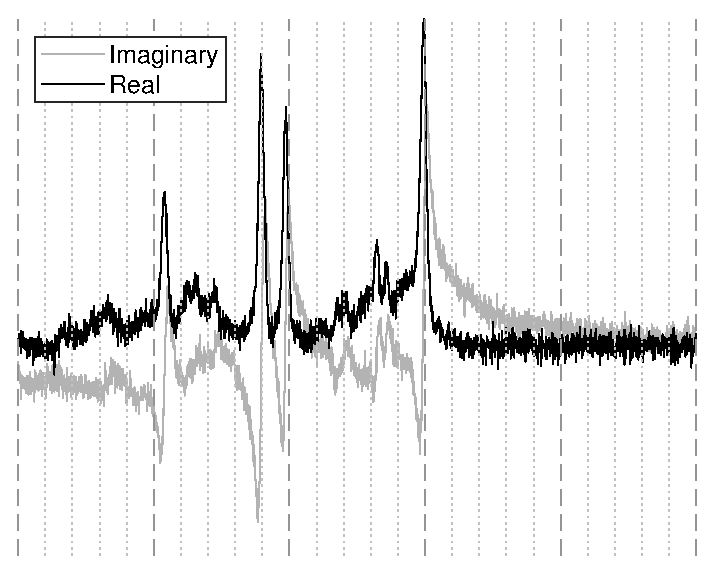
\includegraphics[width=0.95\textwidth,keepaspectratio]{images/phase/no_phase.eps}
        \caption{Spectrum with no phase offsets}
        \label{subfig:no phase}        
    \end{subfigure}
    \begin{subfigure}{0.32\textwidth}
        \centering
        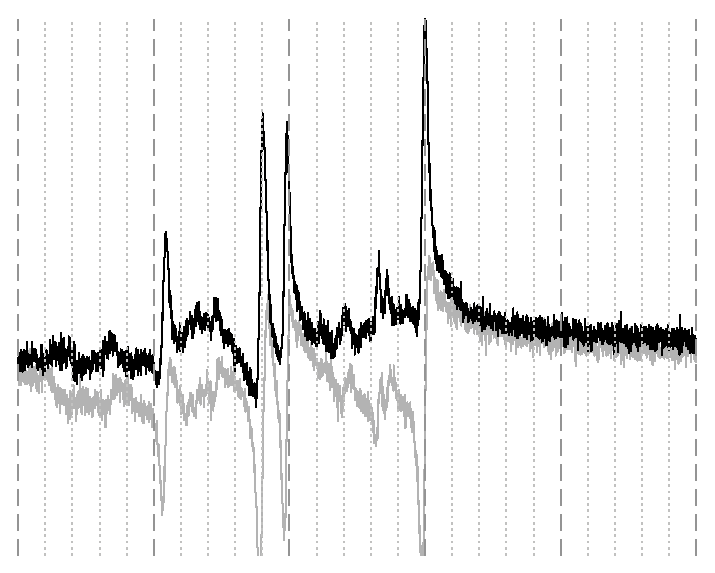
\includegraphics[width=0.95\textwidth,keepaspectratio]{images/phase/zero-order.eps}
        \caption{Spectrum with zero-order phase offset ($\phi_0 = 45^{\circ}$)}
        \label{subfig:zero order phase}        
    \end{subfigure}
    \begin{subfigure}{0.32\textwidth}
        \centering
        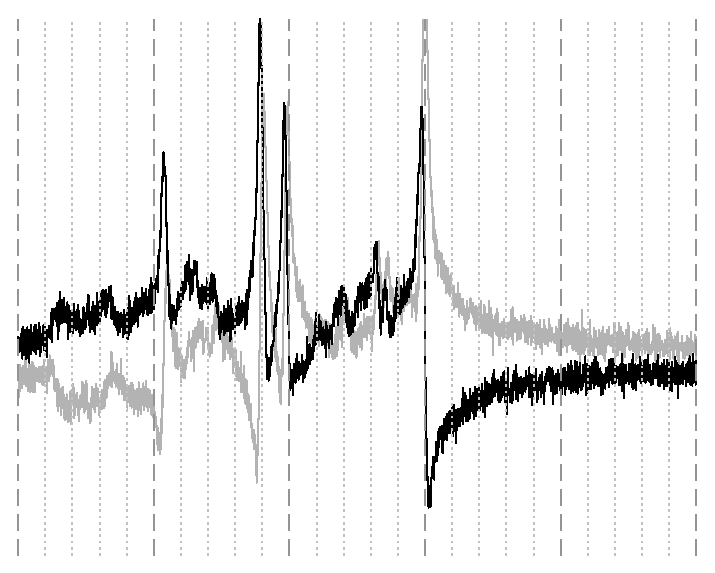
\includegraphics[width=0.95\textwidth,keepaspectratio]{images/phase/first-order.eps}
        \caption{Spectrum with first-order phase offset ($\phi_1 = 20^{\circ}$)}
        \label{subfig:first order phase}        
    \end{subfigure}
    \caption{These samples show how identical spectra are effected by zero- and first-order phase offsets. In \ref{subfig:no phase}, the real component (black) is in absorption mode exhibiting narrow line widths and is fully positive. In \ref{subfig:zero order phase}, a zero-order phase offset is applied. As the spectrum shifts from absorption to dispersion mode, the peaks uniformly lose their symmetry and negative values from the imaginary component are transferred to the real component. In \ref{subfig:first order phase}, a first-order phase shift is applied. This is evident because the asymmetry increases across the spectrum and emanates from the water peak.}
    \label{fig:phase effects}
\end{figure}